% Chapter X

\chapter{Closure laws for the Heat Flux Partitioning model} % Chapter title

\label{ch:HFP_closures} % For referencing the chapter elsewhere, use \autoref{ch:name} 

%----------------------------------------------------------------------------------------


\section{Single-Phase Heat Transfer Coefficient}

The choice of a proper correlation to compute the single-phase heat transfer coefficient is a first but inevitable step to build a HFP model. Indeed, if the single-phase convection term is badly computed, the resulting boiling model will fail to predict the wall temperature.

For instance, if the liquid convective HTC is overestimated, it would result in a delayed increase of the boiling and quenching heat fluxes which would in turn lead to an overprediction of the wall temperature. 

To assess existing correlations for the single-phase HTC, we will use wall temperature measurements extracted from experimental boiling curves for water where $T_{w}\leq T_{sat}$. They correspond to the single-phase part of the experimental data later used to assess the HFP model.

The chosen data are presented on Table \ref{tab:exp_data_convection}.

\begin{table}[h!]

%\begin{changemargin}{-1cm}{0cm}

\noindent\makebox[\textwidth]{

\scriptsize
\centering
\begin{tabular}{p{20mm}|c c c c c c c c} 
Author & $D_{h}$ [mm] & $P$ [bar] & $G_{L}$ [$\debm$] & $\Delta T_{L}$ [K] & $\phi_{w}$ [MW/m\up{2}] & $T_{sat}-T_{w}$ [K] &$N_{mes}$ [-] \\
\hline
\\

Kossolapov \cite{kossolapov_experimental_2021} \newline (2021) & 12 & 10.5 & 500 - 2000 & 10 & 0.1 - 0.6  & 0.22 - 9.5 & 12 \\

Richenderfer \cite{richenderfer_phd} \newline (2018) & 15 & 1 - 5 & 1000 - 2000 & 10-20 & 0.1 - 0.63 & 1 - 18.7 & 13 \\

Jens-Lottes \cite{jens_lottes_data} \newline (1951) & 5.74 & 137.9 & 2617.5 & 53.3 - 92.2 & 0.91 - 2.37 & 0.33 - 44.1 & 15 \\

Kennel \cite{kennel_phd} \newline (1948) & 4.3 - 13.2 & 2 - 6.2 & 284 - 10~577 & 11.1 - 83.3 & 0.035 - 1.89 & 0.35 - 69 & 52 \\
\hline
\end{tabular}
}
\caption{Experimental data range of wall temperature measurements from the single-phase part of boiling curves.}
\label{tab:exp_data_convection}
\end{table}


On Figure \ref{fig:dittus_gniel_htc}, we compare the results of wall temperature prediction in the single-phase region obtained with the correlation of Dittus-Boelter (Eq. \ref{eq:dittus}) and Gnielinski (Eq. \ref{eq:gnielinski}).

\begin{figure}[h!]
\centering
\subfloat[Dittus-Boelter correlation]{
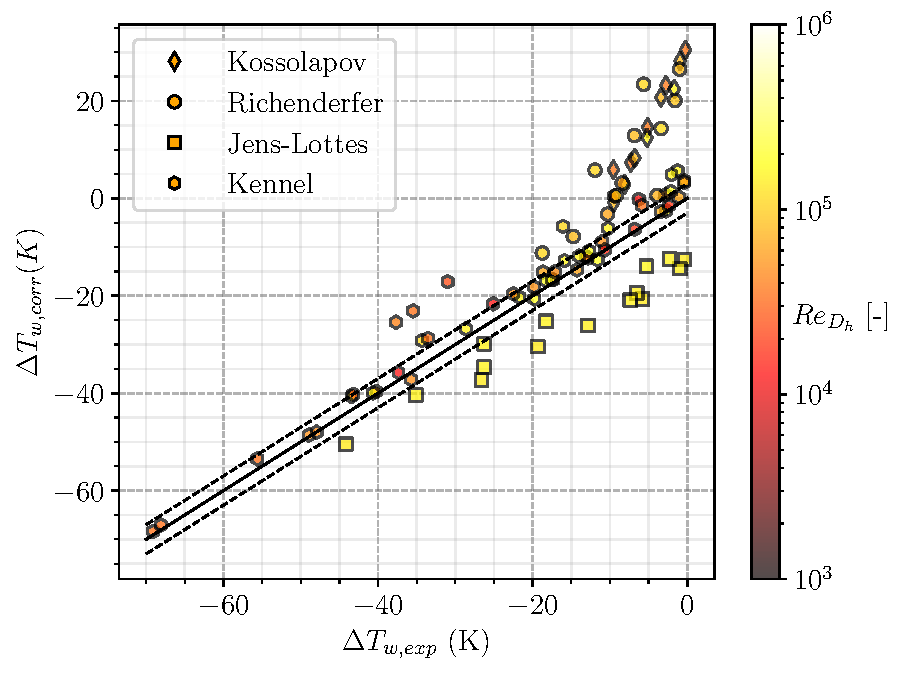
\includegraphics[width=0.45\linewidth]{img/single_phase/comp_dittus.pdf}
\label{fig:dittus_comp}
} 
\subfloat[Gnielinski correlation]{
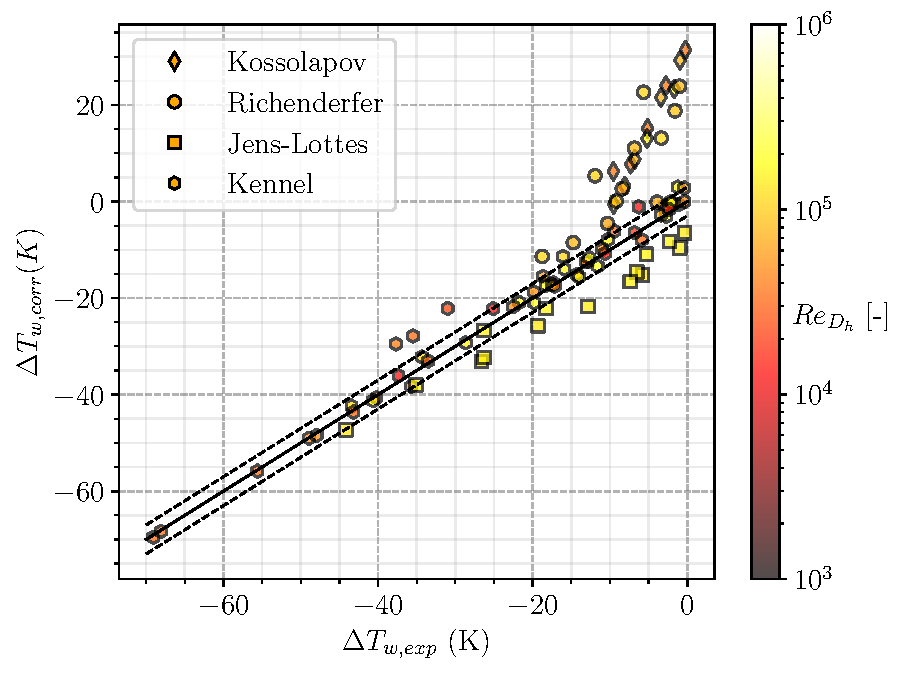
\includegraphics[width=0.45\linewidth]{img/single_phase/comp_gniel.pdf}
\label{fig:gniel_comp}
} 
\caption{Predictive capability of wall temperature by single-phase heat transfer correlations. $\pm 3K$ error bars indicated.}
\label{fig:dittus_gniel_htc}
\end{figure}

The two correlations are of similar efficiency regarding wall temperature predictions over the considered data sets. They both have very good agreement with Kennel data and clear overestimations of $\Delta T_{w}$ on Richenderfer and Kossolapov measurements. The slope difference compared to the parity implies that the correlations are predicting too small Nusselt numbers for those cases. 

Regarding Jens-Lottes data, both model underestimate the wall temperatures, with better results achieved by Gnielinski correlation.

\begin{remark*}{}
We tested different friction factor along with different values of wall roughness in the Gnielinski correlation and observed a negligible impact on the overall results. This allows to stay with a simple formulation for the friction coefficient.
\end{remark*}


The error obtained on Richenderfer and Kossolapov data can be explained by the definition of the HTC computed by Gnielinski correlation. Indeed, Gnielinski correlated a Nusselt number associated to a forced convection coefficient $h_{fc,Gniel}$ in the case of a internal flow with a completely heated wall.

However, only one side of the channel is heated in Richenderfer ans Kossolapov experiments. If $S_{heat}$ denotes this actual heated surface, then Gnielinski correlation estimates the HTC for a surface $4S_{heat}$. With the same imposed total heat power $\Phi_{w}$ and bulk liquid temperature $T_{L}$, we have:

\begin{align}
h_{fc,Gniel} =& \frac{\Phi_{w}}{\parth{T_{w,Gniel}-T_{L}} 4S_{heat}} \\
h_{fc,exp} =& \frac{\Phi_{w}}{\parth{T_{w,exp}-T_{L}} S_{heat}}
\end{align}

Writing $T_{w,Gniel}=T_{w,real}$ then yields:

\begin{equation}
h_{fc,exp}=4h_{fc,Gniel}
\end{equation}

\begin{remark*}{}
This correction can be interpreted as using the thermal diameter instead of the hydraulic diameter, which is 4 times smaller when only one side of the channel is heated.
\end{remark*}

On Figure \ref{fig:ncfd_gniel_corr_htc} we display the predictions of Gnielisnki correlation including this correction by a factor 4 on the HTC for Richenderfer and Kossolapov cases. We also test a $10\%$ reduction on the HTC for Jens-Lottes cases to assess the error made by Gnielinski correlation.

On the same Figure, we also present predictions achieved with the local HTC estimation implemented in NCFD (Eq. \ref{eq:SP_HTC_NCFD}), using a value of $y^{+}=100$. 


\begin{figure}[h!]
\centering
\subfloat[NCFD law]{
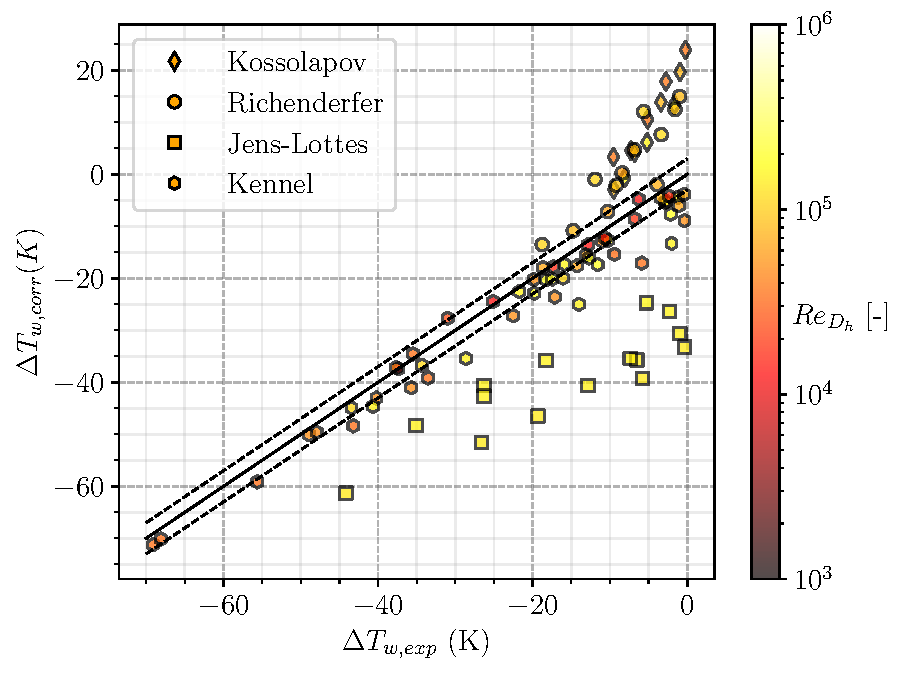
\includegraphics[width=0.45\linewidth]{img/single_phase/comp_ncfd.pdf}
\label{fig:ncfd_comp}
} 
\subfloat[Corrected Gnielinski correlation. We multiply the HTC by 4 on Richenderfer and Kossolapov cases and by 0.9 on Jens-Lotte cases.]{
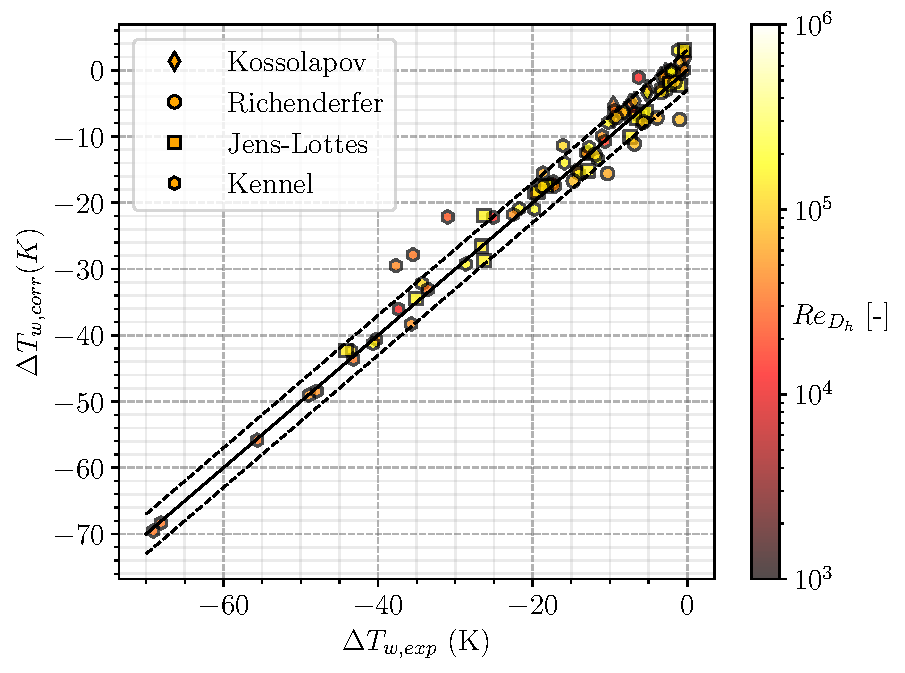
\includegraphics[width=0.45\linewidth]{img/single_phase/comp_gniel_corr.pdf}
\label{fig:gniel_corr_comp}
} 
\caption{Predictive capability of wall temperature by NCFD law and Gnielinski correlation including corrections. $\pm 3K$ error bars indicated.}
\label{fig:ncfd_gniel_corr_htc}
\end{figure}

The NCFD approach yields predictions similar to the 1D correlations (Figure \ref{fig:dittus_gniel_htc}) with larger underestimations on Jens-Lottes measurements. On the other hand, we see that applying a constant correction to the Gnielinski correlation (4 for Kossolapov and Richenderfer cases, 0.9 for Jens-Lottes cases) suffices to yield accurate predictions on the whole range of wall temperature measurements. 

\begin{remark*}{}
The NCFD law was tested without running CFD simulations. The equations were re-written in python to allow its testing outside of the whole code. The use of $y^{+}=100$ as well as the Mac Adams correlation (Eq. \ref{eq:utau_macadams}) for the friction velocity $U_{\tau}$ may induce a difference with the predictions that could be achieved by running a complete CFD computation of the considered cases.
\end{remark*}

The average errors obtained with each model are summed up on Table \ref{tab:error_models_SP_HTC}

\begin{table}[h!]

%\begin{changemargin}{-1cm}{0cm}

\noindent\makebox[\textwidth]{

\scriptsize
\centering
\begin{tabular}{p{25mm}|c c c c c c c c} 
Model & Kossolapov err. [K] & Richenderfer err. [K] & Jens-Lottes err. [K] & Kennel err. [K] \\
\hline
\\

Dittus-Boelter & 19.67 & 15.07 & 10.09 & 3.13 \\
\\

Gnielinski & 20.31 & 14.06 & 6.09 & 1.74 \\
\\

NCFD law & 15.52 & 9.25 & 23.69 & 3.36 \\
\\

Corrected Gnielisnki & 1.34 & 3.08 & 1.57 & 1.74 \\
\\

\hline
\end{tabular}
}
\caption{Average errors achieved by the considered models on each data sets.}
\label{tab:error_models_SP_HTC}
\end{table}


\textbf{Recalling that Gnielinski correlation was also providing good results on the DEBORA cases with R12 (Chapter \ref{chap:debora}), this further indicates it as a proper choice regarding single-phase HTC estimation in the HFP model.} However, we will later allow the use of the correction factors when needed to ensure a proper representation of the single-phase part when trying to assess the models associated to boiling.




\section{Single Bubble Quenching Area}

When computing the quenching heat flux, we need to provide the total wall area visited by a single bubble $A_{q,1b}$ that will undergo quenching.

In wall boiling model that do not consider bubble sliding \cite{kurul_podowski, ncfd_hfp, shaver_podowski} the impacted area at bubble lift-off is often considered as :

\begin{equation}
A_{q,1b} = F_{A} \pi R_{lo}^{2}
\end{equation} 
with $F_{A}$ being an enhancement factor that accounts for the the possibility that the bubble will induce quenching over a surface larger than its projected area.



\begin{align}
A_{q,1b} = &
\begin{dcases}
\pi R_{lo}^{2} & \text{if } l_{sl}\leq R_{lo}-R_{d} \\
%
\frac{1}{2}\pi R_{d}^{2} + l_{sl}\parth{R_{d}+R_{lo}} + \frac{1}{2}\pi R_{lo}^{2} & \text{if } l_{sl} \geq R_{lo}+R_{d}
%
\end{dcases}
\end{align}

Which can be re-expressed by defining ${l_{sl}}^{*}=\dfrac{l_{sl}}{R_{lo}}$ and ${A_{q,1b}}^{*}=\dfrac{A_{q,1b}}{\pi R_{lo}^{2}}$

\begin{align}
{A_{q,1b}}^{*} = &
\begin{dcases}
1 & \text{if } {l_{sl}}^{*}\leq 1- \frac{R_{d}}{R_{lo}} \\
%
\frac{1}{2}\parth{1+\parth{\frac{R_{d}}{R_{lo}}}^{2} } + \frac{{l_{sl}}^{*}}{\pi}\parth{1+\frac{R_{d}}{R_{lo}}} & \text{if } {l_{sl}}^{*} \geq 1 + \frac{R_{d}}{R_{lo}}
\end{dcases}
\end{align}
and we linearly interpolate those two expressions for the region where $1-\dfrac{R_{d}}{R_{lo}}\geq {l_{sl}}^{*} \geq 1+\dfrac{R_{d}}{R_{lo}}$.


\section{Growth time}




In this case, the average radius of the bubble over a growth time $t_{g}$ (as needed in Subsection \ref{subsec:vap_area}) is :


\begin{align}
\overline{R\parth{t}}&=\frac{1}{t_{g}}\int_{0}^{t_{g}}R\parth{t} \text{d}t = \frac{R_{\infty}}{t_{g}}\crocht{ \frac{e^{-2K_{a}\sqrt{t}} \parth{2K_{a}\sqrt{t}+1}  }{2K_{a}^{2}}+ t}_{0}^{t_{g}}\\
&=\frac{R_{\infty}}{2K_{a}^{2}t_{g}}\parth{ e^{-2K_{a}\sqrt{t_{g}}}\parth{2K_{a}\sqrt{t_{g}}+1} + 2K_{a}^{2}t_{g} -1  }
\end{align}

Moreover, if we consider a lift-off radius $R_{d}$, we can express the associated growth time $t_{g}$ :

\begin{align}
t_{g}=\crocht{ \frac{1}{K_{a}}\ln{\frac{1}{\sqrt{1-\frac{R_{d}}{R_{\infty}} } } } }^{2} = \crocht{\frac{1}{K_{a}}\ln { \sqrt{1-\frac{R_{d}}{R_{\infty}} } }   }^{2}
\label{eq:growth_time}
\end{align}

This expression could then be used as a closure relationship for $t_{g}$ in the HFP model, meaning that this growth time will depend on the departure diameter closure for $R_{d}$.


\subsection{Estimation of the thermal boundary layer thickness $\delta$}

In order to fully close the modeling of the bubble growth, we have to compute the thermal boundary layer thickness $\delta$.

To do so, we test a first approach based on the hydrodynamic boundary layer profile. In the turbulent layer, the non-dimensional liquids velocity $u_{l}^{+}$ is :

\begin{align}
u_{l}^{+}=\frac{1}{\kappa} \ln{y^{+}} +B,\ \text{with}\ \kappa=0.41\ \text{and}\ B=5.25
\end{align}

Since $u_{l}^{+}\parth{y^{+}}=u_{l}\parth{y}/u_{\tau}$ and $y^{+}=yu_{\tau}/\nu_{l}$, we can compute the height of the hydrodynamic boundary layer $\delta_{h}$ where $u_{l}\parth{\delta_{h}}=0.99u_{l,bulk}$ as :

\begin{align}
\delta_{h}=e^{\kappa \parth{0.99u_{l,bulk}\sqrt{\rho_{l}/\tau_{w}}-B}}\times \nu_{l}\sqrt{\frac{\rho_{l}}{\tau_{w}}}
\end{align}

where $\tau_{w}$ is computed using the Mac Adams correlation (Eq. \ref{eq:MacAdams}).

\npar

Finally, to get an approximation of the thermal boundary layer thickness, we consider a simple first approach as :

\begin{align}
\delta=\frac{1}{\Pr_{l}}\delta_{h}
\end{align}

Since the Prandtl number is the ratio of momentum diffusivity to thermal diffusivity, its inverse shall approximately scale the ratio between the thermal boundary layer and hydrodynamic boundary layer thickness. 

\npar

\subsection{Estimation of $t{g}$ against experimental data}

In order to assess the proposed approach to compute $t_{g}$, we compare the yielded results with data taken from Unal of maximum bubble growth. 

\npar

Only 6 measurements of maximum growth time are available ({\color{red} Je vais en ajouter d'autres par la suite}) but they are associated with the bubble lift-off diameter. Since those measurements were conducted with boiling water on stainless steel, we set the contact angle at $\alpha=80\degree$.

\npar

We also compare the predictions with the model proposed by Kommajosyula :

\begin{align}
t_{g}&=\parth{ \frac{D_{d}}{4K}}^{2}\\
K&=\frac{\sqrt{\eta_{l}} \Ja_{w}}{0.804\sqrt{\Pr_{l}}}+\chi 1.95\Ja_{w} \eta_{l},\ \text{with}\ \chi=A-B\zeta
\end{align}
where $\zeta=\Ja_{l}/\Ja_{w}$ and both $A=1.55$ and $B=0.05$ have been fitted over the data of Klausner by Mazzocco \etal.

\npar

The results are displayed on Figure \ref{fig:comp_modelKomm}.

\begin{figure}[h!]
\centering
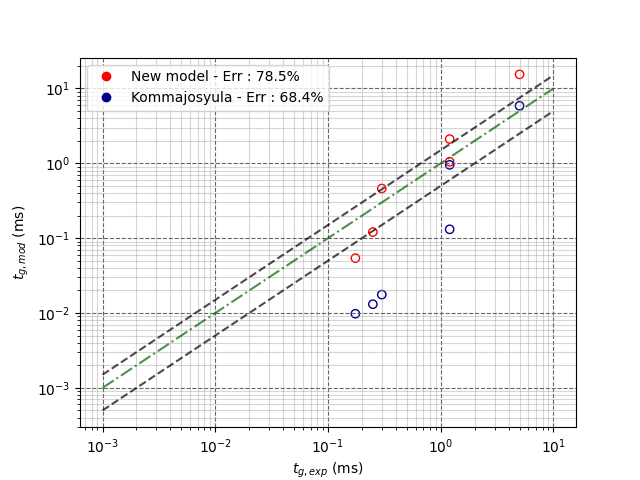
\includegraphics[width=0.6\linewidth]{img/tg/comp_tg_unal.png}
\caption{Comparison of the proposed model and Kommajoyusla model against experimental data from Unal. Black lines represent the $\pm 50\%$ error bars.}
\label{fig:comp_modelKomm}
\end{figure}

As we can see, the average error from our model is greater than Kommajosyula's one. However, this is mainly due to the highest measured growth time (upper right point). Without this measurement, the average error reaches $52.5\%$, indicating that a much greater number of experimental measurements should be needed properly evaluate each model.

\npar
On the other hand, we may consider that the proposed approach could be of interest since it is not based on data-fitted parameters while providing reasonable results.



\begin{table}[h!]

%\begin{changemargin}{-1cm}{0cm}

\noindent\makebox[\textwidth]{

\scriptsize
\centering
\begin{tabular}{p{20mm}|c c c c c c c c} 
Author & Fluid & $D_{h}$ [mm] & $P$ [bar] & $G_{L}$ [$\debm$] & $\Delta T_{L}$ [K] & $\phi_{w}$ [kW/m\up{2}] & $\Delta T_{w}$ [K] & $D_{d}$ [mm] ($N_{mes}$)\\
\hline
\\

Maity \cite{maity_effect_2000} \newline (2000) & Water & 20 & 1.01 & 0 - 239.6 & 0.3 - 0.7 & N.A. & 5 - 5.9 & 0.788 - 1.71 (9) \\

Kossolapov \cite{kossolapov_experimental_2021} \newline (2021) & Water & 20 & 20 - 40 & 500 - 1500 & 0.3 - 0.7 & N.A. & 5 - 5.9 & 0.788 - 1.71 (9) \\

\hline
\end{tabular}
}


\caption{Bubble growth time data in vertical flow boiling}
\label{tab:tg_exp_data}

%\end{changemargin}

\end{table}

\section{Bubble Wait Time}

The wait time between two nucleation events on an active site corresponds to the time needed for the thermal boundary layer to reconstruct after its disruption due do bubble departure from the nucleation site.  
\begin{table}[h!]

%\begin{changemargin}{-1cm}{0cm}

\noindent\makebox[\textwidth]{

\scriptsize
\centering
\begin{tabular}{p{20mm}|c c c c c c c c} 
Author & Fluid & $D_{h}$ [mm] & $P$ [bar] & $G_{L}$ [$\debm$] & $\Delta T_{L}$ [K] & $\phi_{w}$ [kW/m\up{2}] & $\Delta T_{w}$ [K] & $D_{d}$ [mm] ($N_{mes}$)\\
\hline
\\

Basu \etal \cite{basu_heat} \newline (2005) & Water & 20 & 1.01 & 0 - 239.6 & 0.3 - 0.7 & N.A. & 5 - 5.9 & 0.788 - 1.71 (9) \\
\\

Richenderfer \etal \cite{richenderfer_investigations_2018} \newline (2018) & Water & 20 & 1.01 & 0 - 239.6 & 0.3 - 0.7 & N.A. & 5 - 5.9 & 0.788 - 1.71 (9) \\
\\

Kossolapov \etal \cite{kossolapov_experimental_2021} \newline (2021) & Water & 20 & 1.01 & 0 - 239.6 & 0.3 - 0.7 & N.A. & 5 - 5.9 & 0.788 - 1.71 (9) \\
\\
\hline
\end{tabular}
}

\caption{Bubble wait time data in vertical flow boiling}
\label{tab:tw_exp_data}


%\end{changemargin}

\end{table}



Formulation of Basu \etal \cite{basu_heat_2005}:

\begin{equation}
t_{w} = 139.1\Delta {T_{w}}^{-4.1}
\end{equation}


Formulation of Kommajosyula \cite{komma}:

\begin{equation}
t_{w} = 0.061\frac{{\Ja_{L}}^{0.63}}{\Delta T_{w}}
\end{equation}

\begin{remark*}
Kommajosyula's correlation yields a zero wait time when bulk liquid approaches saturation. This behavior is questionable 
\end{remark*}

Mikic \& Rosenhow analytical expression \cite{mikic}:

\begin{align}
t_{w} = \frac{1}{\pi \eta_{L}}\crocht{ \frac{\parth{\Delta T_{w}+ \Delta T_{L}}R_{c}}{\Delta T_{w} - T_{sat} \parth{\dfrac{1}{\rho_{V}}-\dfrac{1}{\rho_{L}}} \dfrac{2\sigma}{h_{LV}R_{c}} } }^{2}
\end{align}

A relevant


\section{Nucleation Site Density}

The Nucleation Site Density is among the most influencing parameters over the HFP models predictions, particularly regarding wall temperature. Indeed, its value directly controls the density of bubbles generated at the heater and therefore impacts both the boiling ($\phi_{e}$) and quenching ($\phi_{q}$) heat fluxes to the first order. Being able to come up with correct predictions of the NSD is thus critical if one wishes to properly capture the thermal behavior of the boiling surface.

However, the value of $N_{sit}$ is actually influenced by many parameters being either linked to thermal-hydraulics (wall temperature, pressure, operating fluid) or the heater material (roughness, wettability). That is why its value is often estimated through empirical correlations, for which many different expression have been proposed over the years since the end of the XX\textsuperscript{th} century.

\npar

One of the firstly identified behavior of the NSD was its power dependency with the wall superheat ($N_{sit} \propto {\Delta T_{w}}^{m}$), which is form adopted in the correlation of Lemmert \& Chawla \cite{lemmert} : 

\begin{align}
N_{sit}=\crocht{210\parth{T_{w}-T_{sat}}}^{1.8}
\label{eq:nsit_lemmert}
\end{align}

\begin{remark*}{}
This law is used in the HFP model of Kurul \& Podowski and NEPTUNE\_CFD to compute $N_{sit}$.
\end{remark*}

However, such an expression misses the influence of other parameters such as pressure, which has been proven to be strongly impacting the range of active cavities that can generate bubbles as shown on Figure \ref{fig:nsd_P_koss} and induces a larger bubble density over the heater. 

\begin{figure}[h!]
\centering
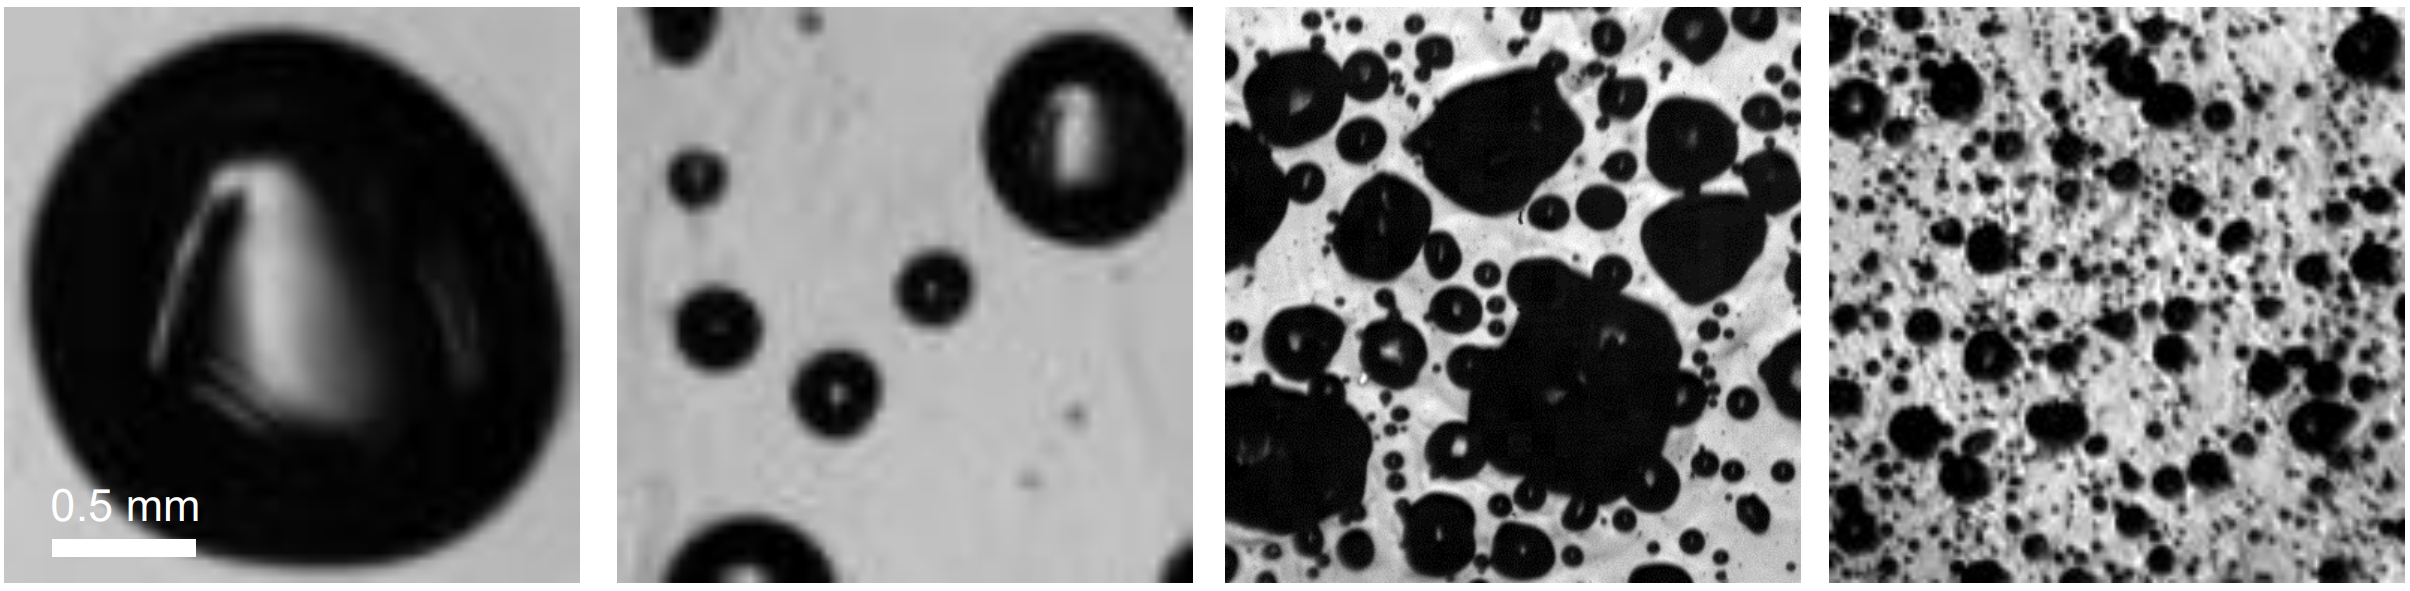
\includegraphics[width=0.7\linewidth]{img/NSD/nsd_press_koss.png}
\caption{HSV Visualization of bubble density at various pressures adapted from Kossolapov \cite{kossolapov_experimental_2021} (left to right: 1.01 bar, 3 bar, 19.8 bar, 75.8 bar). }
\label{fig:nsd_P_koss}
\end{figure}

\npar

Moreover, experimental measurements such as in Borishanskii \cite{borishanskii} showed that the power dependency on the wall superheat changes by increasing both with pressure and the superheat value itself. This was accounted for by Hibiki \& Ishii in 2003 \cite{hibiki_ishii} who came up with a new correlation that requires an estimation of the minimum activated cavity radius $R_{c}$ : 


\begin{align}
N_{sit} =& N_{0}\parth{1-\exp{-\dfrac{\theta^{2}}{8\mu^{2}} } }\crocht{\exp{ \mathrm{f}\parth{\rho^{+}}\dfrac{\lambda '}{R_{c}} } -1}
\label{eq:nsit_hibiki} \\
%
R_{c} =& \dfrac{2\sigma\parth{1+\dfrac{\rho_{V}}{\rho_{L}}} / P }{\exp{\dfrac{h_{LV} \Delta T_{w}}{R_{g}T_{w}T_{sat}} } -1}\\
%
\mathrm{f}\parth{\rho^{+}} =& -0.01064 + 0.48246\rho^{+} - 0.22712 \rho^{+^{2}} + 0.05468 \rho^{+^{3}}
\end{align}
with $R_{g}$ the perfect gas constant times the molar mass of the fluid,  $N_{0}=4.72\times 10^{5}\ \mathrm{m}^{-2}$, $\mu = 0.722\ \mathrm{rad}$, $\lambda ' = 2.5 \times 10^{-3} \ \mathrm{m}$ and $\rho^{+}=\mathrm{log}_{10}\parth{\dfrac{\rho_{L}-\rho_{V}}{\rho_{V}}}$.


\begin{remark*}{}
This law is used in the HFP model of Gilman \& Baglietto \cite{gilman_baglietto}.
\end{remark*}

We can note that it also includes the value of the static contact angle $\theta$ which can be used as a parameter to accounts for wall properties, since it is dependent on the wall roughness, wettability and the operating fluid. 

Indeed, a high-wetting material (low values of $\theta$) will allow smaller cavities to be flooded by the surrounding liquid, thus hindering non-condensable gases to be captured inside and become a potentially active nucleation site (Figure \ref{fig:nsd_theta_wet}).

\begin{figure}[h!]
\centering
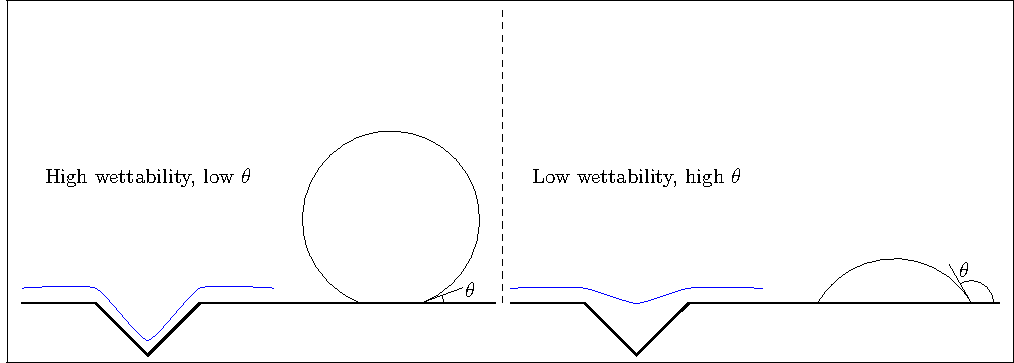
\includegraphics[scale=0.8]{img/NSD/wettability.pdf}
\caption{Sketch of the link between bubble contact angle and wettability / cavity flooding}
\label{fig:nsd_theta_wet}
\end{figure}

This influence of the contact angle on the NSD was confirmed by experimental obervations of Basu \etal \cite{basu_nsit} and was also included in a law correlated on their own measurements :

\begin{align}
N_{sit}=&
\begin{dcases}
0.34\crocht{1-\cos{\theta}} {\Delta T_{w}}^{2} & \text{if } \Delta T_{w,ONB}<\Delta T_{w} < 15\ K\\
3.4\times 10^{-5}\crocht{1-\cos{\theta}} {\Delta T_{w}}^{5.3} & \text{if } \Delta T_{w} > 15\ K
\end{dcases}
\label{eq:nsit_basu}
\end{align}

\npar

Similarly, Zhou \etal \cite{zhou_nsd} correlated their measurements, including an influence of the pressure:

\begin{align}
N_{sit} =& N_{0}\parth{1-\cos{\theta}}\crocht{\exp{\mathrm{f}\parth{P} \Delta T_{w} } -1 }
\label{eq:nsit_zhou}\\
&\mathrm{f}\parth{P} = 0.218~\ln{\dfrac{P}{P_{0}}}+0.1907
\end{align}
with $N_{0}=55~395.26\ \mathrm{m}^{-2}$ and $P_{0}=1.01\ \mathrm{bar}$.

\npar

Finally, one of the most recent NSD correlation has been proposed by Li \etal in 2018 \cite{li_new_2018} and validated over a large range of measurements by including a more realistic power law for $\Delta T_{w}$. It avoids the divergence of $N_{sit}$ observed in Hibiki \& Ishii law (Eq. \ref{eq:nsit_hibiki}) when reaching high pressure and superheats. It also includes the impact of pressure and contact angle and its evolution with temperature \eg its decrease close to 0 $\degree$ when approaching the critical temperature \cite{song_fan_contact_angle}:


\begin{align}
N_{sit} &= N_{0}e^{\mathrm{f}\parth{P}} {\Delta T_{w}}^{A\Delta T_{w} + B} \parth{1- \cos{\theta}}
\label{eq:nsit_li}\\
%
\mathrm{f}\parth{P} &= 26.006 - 3.678 e^{-2P} - 21.907e^{-P / 24.0.65}\\
%
A &= -2\times 10^{-4} P^{2} + 0.0108P + 0.0119\\
%
B &= 0.122P +1.988\\
%
1-\cos{\theta} &= \parth{1-\cos{\theta_{0}}}\parth{\frac{T_{c}-T_{sat}}{T_{c}-T_{0}}}^{\gamma}
\end{align}
with $P$ in MPa, $\theta_{0}$ the contact angle at room temperature $T_{0}$, and default value being for water $\theta_{0}=41.37 \degree$, $T_{c}=374 \degree$C $T_{0}=25\degree$C, $\gamma = 0.719$.

\begin{remark*}{}
We can question the absence of bulk liquid velocity and temperature in the presented law since they should logically influence the nucleation process. However, this impact is rather limited as observed in experimental measurements of Zhou \etal and Kossolapov.
\end{remark*}

\npar

In order to assess existing NSD correlations and choose the most pertinent to include in a HFP model, we gather NSD measurements from 4 different authors. The different operating conditions of the chosen data sets are gathered on Table \ref{tab:nsit_exp_data}.


\begin{table}[h!]

%\begin{changemargin}{-1cm}{0cm}

\noindent\makebox[\textwidth]{

\scriptsize
\centering
\begin{tabular}{p{20mm}|c c c c c c c c} 
Author & Fluid &  $P$ [bar] & $G_{L}$ [$\debm$] & $\Delta T_{L}$ [K]  & $\Delta T_{w}$ [K] & $\theta_{0}$ [$\degree$] &  $N_{mes}$ [-]\\
\hline
\\

Zhou \cite{zhou_nsit} \newline (2020) & Water & 1.21 - 3.12 & 482.7 - 1930.6 & 8 - 15  & 6.7 - 20.2 & $51$ & 60 \\
\\

Richenderfer \cite{richenderfer} \newline (2018) & Water & 1.01 & 500 - 1000 & 10 & 21.7 - 42.8 & $80$ & 49 \\
\\

Kossolapov \cite{kossolapov_experimental_2021} \newline (2021) & Water & 1.01 - 75.8 & 500 - 2000 & $80$ &10 & 80\degree & 63 & \\
\\

Borishanskii \cite{borishanskii} \newline (1966) & Water & 1.01 - 198 & N.A. & N.A. & 1.75 - 17.3 & $45$ & 132 \\
\\

\hline
\end{tabular}
}

\caption{Nucleation Site Density data in flow boiling}
\label{tab:nsit_exp_data}


\end{table}



We then compare the predictions achieved by the model of Lemmert \& Chawla (Eq. \ref{eq:nsit_lemmert}), Hibiki \& Ishii (Eq. \ref{eq:nsit_hibiki}), Zhou \etal (Eq. \ref{eq:nsit_zhou}) and Li \etal (Eq. \ref{eq:nsit_li}).  The comparison with measurements are presented on Figure \ref{fig:pred_nsit_models}.




\begin{figure}[!h]
\centering
\subfloat[Lemmert \& Chawla model]{
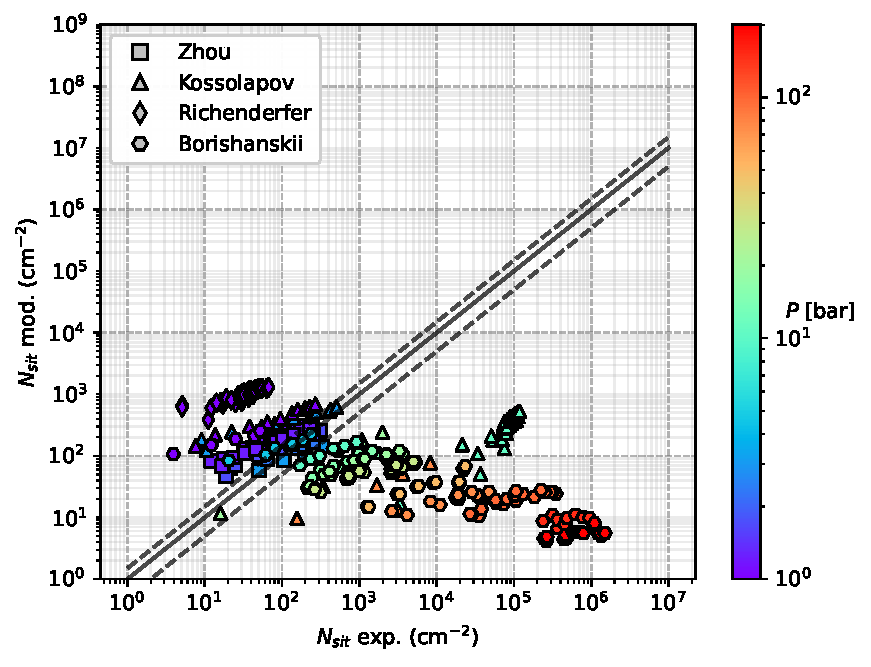
\includegraphics[width=0.45\linewidth]{img/NSD/nsit_LC.pdf}
\label{fig:pred_nsit_lemmert}
} 
\subfloat[Hibiki \& Ishii model]{
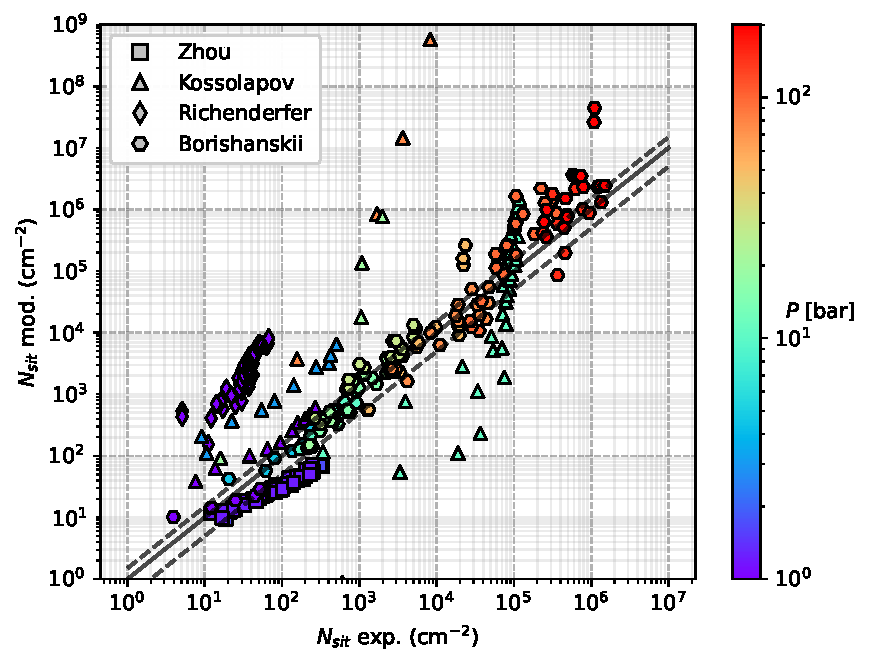
\includegraphics[width=0.45\linewidth]{img/NSD/nsit_HI.pdf}
\label{fig:pred_nsit_hibiki}
}
\\
\subfloat[Zhou \etal model]{
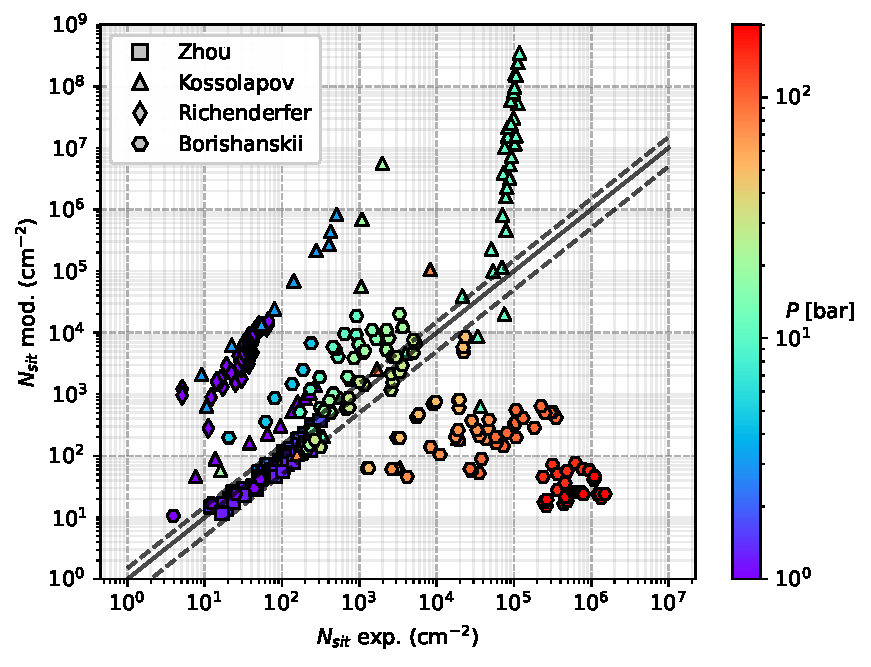
\includegraphics[width=0.45\linewidth]{img/NSD/nsit_Zhou.pdf}
\label{fig:pred_nsit_zhou}
} 
\subfloat[Li \etal model]{
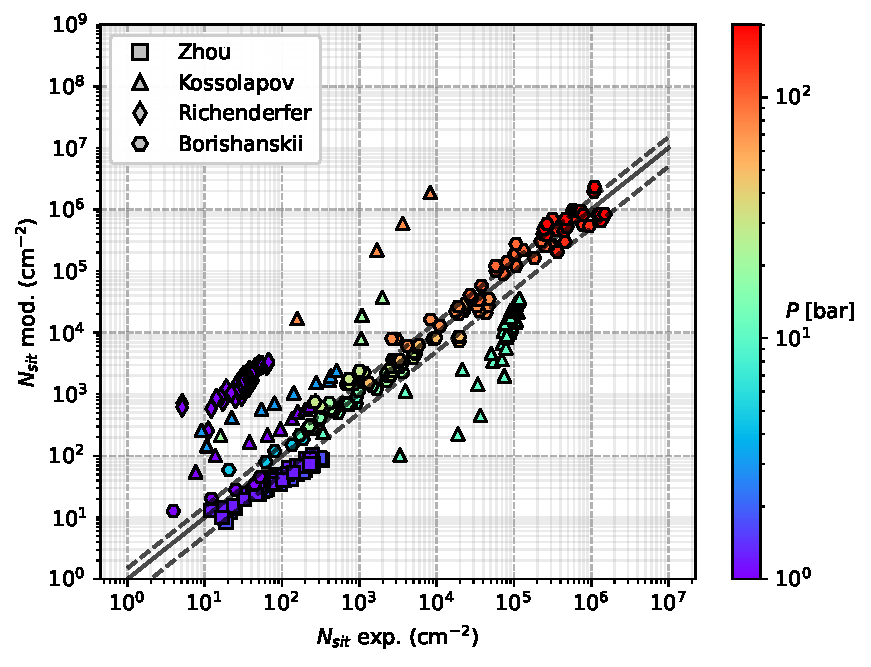
\includegraphics[width=0.45\linewidth]{img/NSD/nsit_Li.pdf}
\label{fig:pred_nsit_li}
}

\caption{Predictions of the chosen models against the experimental data of Table \ref{tab:nsit_exp_data} with $\pm 50\%$ error bars. The contact angles}
\label{fig:pred_nsit_models}
\end{figure}

The Lemmert \& Chawla model appears to fail in predicting the NSD at high pressures. This is a logical drawback of its sole dependence on the wall superheat. More importantly it increasingly underestimates the NSD as pressure increases, which makes it a clearly unsuitable correlation to compute $N_{sit}$ particularly for pressurized flows such as in PWR.

Altough the model of Zhou \etal includes a pressure term, its partial calibration on data covering a low range of pressure may explain the large error observed when compared to higher pressure measurements.

On the contrary, models from Hibiki \& Ishii and Li \etal seem to better reproduce the different trends with flow conditions, especially with pressure. The model from Li \etal achieves better predictions by avoiding to reach unphysically high values of $N_{sit}$ at higher wall superheat compared to Hibiki \& Ishii. This behavior is clear over Kossolapov data at high pressure, where both model lead to overestimations, the strongest discrepancy being associated to Hibiki \& Ishii model.

Overall, the model of Li \etal is the most efficient with an acceptable agreement on most of the data of Borishanskii and Zhou \etal. The measurements of Richenderfer and Kossolapov fail to be precisely reproduced, but it shows a coherent trend and the most limited error when compared to other correlations.

\begin{remark*}{}
The coherency of NSD predictions is hard to ensure since we do not know the exact contact angle and boiling surface morphology in the experiments. This was pointed out by Richenderfer \cite{Richen_phd} who observed significant variation in the NSD value depending on the heater, though keeping the same material (ITO). For instance, this may explain the fact that the NSD measured by Kossolapov at $10.5$ bar is higher than any other pressure on his experiment, leading to both underpredictions and overpredictions of the model of Li \etal depending on the pressure.
\end{remark*}


All things considered, those comparisons show that the Nucleation Site Density remains among the most difficult quantity to evaluate because of its very large variations over experiments, boiling surfaces and flow conditions. Dedicated correlations are hardly precise outside of their establishment databases. However, it remains the best yet only way to compute $N_{sit}$. \textbf{In that regard, the NSD correlation of Li \etal appears to be the most coherent choice.}


\section{Considerations on bubble interaction and nucleation sites deactivation}

NSD correlation actually compute the total number of sites where bubbles can nucleate on a surface. However, they do not represent how important a nucleation site will be in term of bubbles generation compared to another. 

\npar
In fact, Kossolapov has observed that each nucleation site has its own bubble nucleation frequency. Thus implying that some sites play a much greater role in wall nucleation compared to others. One can even consider that some nucleation sites can be neglected regarding their small impact on the whole phase change process.

\npar

In order to physically take into account this effect, Gilman considered a statistical approach, by assuming that nucleation site are randomly distributed over the heater surface (Complete Spatial Randomness). Then, considering that a nucleation site located under a bubble will be deactivated, one can express the number of sites actually contributing to bubble nucleation $N_{sit,a}$ as :


\begin{align}
N_{sit,a}=\parth{1-\mathcal{P}}N_{sit},\ \text{with}\ \mathcal{P}=1-e^{-N_{b}\pi \parth{D_{b}/2}^{2}}
\end{align}
where $N_{b}=t_{g}fN_{sit}$ is the actual average density of bubbles on the heater surface.

\npar

The resulting number of sites is a solution of the implicit equation on $N_{sit}$, which can be solved numerically or using the Lambert function (reciprocal of $w\rightarrow we^{-w}$).

\npar

{\color{red} Je vais détailler un peu plus cela avec des schémas clairs, ainsi qu'un exemple de comment cela pondère la densité de site totale, puisque cela permet d'éviter la divergence dans une loi telle que celle de Hibki \& Ishii à haute surchauffe pariétale} 


\subsection{Static suppression}

If we suppose that the nucleation sites follow a homogeneous spatial Poisson process with an event density $\lambda$, we can express the probability of finding $n$ sites within an area A as :

\begin{align}
\mathcal{P}\parth{N\parth{A}=n}=\frac{\parth{\lambda A}^{n}}{n!}e^{-\lambda A}
\end{align}

If we consider the actual number of bubble-generating sites $N_{b}$, those sites are holding a bubble over a fraction $t_{g}f$ of the nucleation cycles in average. Thus, the actual density of bubbles held by the sites is : $t_{g}f N_{b}$. To derive $N_{b}$ from the value $N_{sit}$ provided by NSD correlations, we have to evaluate the probability of nucleation site overlapping, which corresponds to a distance $r$ lower than $R_{d}$ between two bubbles. 

\begin{align}
\mathcal{P}\parth{r\leq R_{d}} &=1-\mathcal{P}\parth{N\parth{\pi R_{d}^{2}}=0}\\
&=1-e^{-N_{b}t_{g}f\pi R_{d}^{2}} = \mathcal{P}
\end{align}

This probability thus represents the proportion of bubble that can't be geometrically accomodated on the surface. We can then evaluate $N_{b}$ from $N_ {sit}$ as :

\begin{align}
&N_{b}=\parth{1-\mathcal{P}}N_{sit} \\
%
\Leftrightarrow\  &N_{b}t_{g}f\pi R_{d}^{2}e^{N_{b}t_{g}f \pi R_{d}^{2}}= N_{sit}t_{g}f \pi R_{d}^{2} \\
%
\Leftrightarrow\   &N_{b} = \frac{\mathcal{W}\parth{N_{sit}\mathsf{A}}}{\mathsf{A}}\ \ \ \text{where}\ \ \ \mathsf{A}=t_{g}f\pi R_{d}^{2}
\end{align}



\subsection{Static coalescence}

Now that the actual number of bubble-generating sites have been identified, we can consider other interaction phenomena that can occur on the boiling surface. For instance, if two sites are simultaneously generating a bubble at a distance $d$ between $R_{d}$ and $2R_{d}$, the bubbles will coalesce while growing up to the detachment diameter. To estimate the probability of having a bubble on a site in this distance range, we consider the probability density function of the nearest-neighbour in the case of a homogeneous spatial Poisson process $f$ with an event density $\lambda$. 

\begin{align}
f\parth{r}=2\lambda \pi r e^{-\lambda \pi r^{2}}
\end{align} 

The considered probability of interaction is then :

\begin{align}
\mathcal{P}\parth{R_{d}\leq r \leq 2R_{d}} &=\int_{R_{d}}^{2R_{d}}f\parth{r} \mathrm{d}r \\
%
&= e^{-\lambda \pi R_{d}^{2}} - e^{-4\lambda \pi R_{d}^{2}}\\
%
&= e^{-\lambda \pi R_{d}^{2}}\crocht{1-\parth{e^{-\lambda \pi R_{d}^{2}}}^{3}} \\
&= \mathcal{P}_{coal,st} \ \ \ \text{with}\ \ \ \lambda=t_{g} f N_{b}
\end{align}

The density of bubble-generating sites that will lead to a static coalescence can then be estimated as :

\begin{align}
N_{coal,st}=\mathcal{P}_{coal,st}N_{b}
\end{align}

If we suppose that coalescing bubbles will instantly lift-off due to the perturbation associated with the coalescence process, this yields an associated boiling flux :

\begin{align}
\phi_{e,coal,st}=N_{coal,st} f \rho_{V}h_{LV} \frac{4}{3}\pi R_{coal,st}^{3} \ \ \ \text{where}\ \ \ R_{coal,st}=\sqrt[3]{2}R_{d} 
\end{align}

considering that the bubbles will merge approximately at $R=R_{d}$.

\subsection{Sliding coalescence}

Now that suppressed sites and sites that will lead to static coalescence have been identified, the remaining sites $N_{sl}=\parth{1-\mathcal{P}_{coal,st}}N_{b}$ will generate sliding bubbles. While sliding, a single bubble swipes an area :

\begin{align}
A_{sl, 1b} \approx l_{sl,1b}\frac{D_{d}+D_{lo}}{2}
\end{align}

In this area, there are an average number of bubble-generating sites $N_{b}A_{sl,1b}$ and an average number of growing bubbles on their sites $t_{g}f N_{b}A_{sl,1b}$

\npar
Two situations can happen from the sliding process :

\begin{itemize}
\item The bubble slides without coalescing
\item The bubble coalesces while sliding with a bubble growing on its site and lifts-off
\end{itemize}


Following the same approach from the static suppression, we can estimate the probability of finding no growing bubble over the sliding surface : 

\begin{align}
\mathcal{P}\parth{N\parth{A_{sl,1b}}=0 }=e^{-N_{b}t_{g}fA_{sl,1b}}
\end{align}

Thus, if a sliding bubble among the $N_{sl}$ does not encounter any growing bubble, the sites on its sliding area will be wiped and thus be quenched by cold liquid. This means that those sites will be suppressed due to the sliding of other bubbles over them.

Among the $N_{b}$ bubble generating sites we can identify 4 categories of sites :

\begin{itemize}
\item Sites generating bubbles which will slide without encountering any growing bubble on their path : $$N_{sl, NC}=N_{sl}e^{-ft_{g}N_{b}A_{sl,1b}}$$

\item Sites generating bubbles that will coalesce with a growing bubble during sliding : 
$$N_{sl, C}=  N_{sl}\parth{1-e^{-ft_{g}N_{b}A_{sl,1b}}}$$

\item Sites which will be suppressed by bubbles sliding without coalescing : $$N_{sup, sl}=N_{sl,NC}\ N_{b}A_{sl,1b}$$

\item Sites generating bubbles that will coalesce with a sliding bubble coming from upstream. Those bubbles are still in the growing phase up to detachment when they are coalescing with sliding bubbles. Therefore, there are equal to the number of sliding bubbles that will coalesce : $$N_{g,C}=N_{sl,C}$$

\end{itemize}

This allows to finally write :

\begin{align}
N_{b}&=N_{sl,NC}+N_{sl,C}+N_{sup,sl} + N_{g,C}\\
%
&=N_{sl}\crocht{2-e^{-ft_{g}N_{b}A_{sl,1b}}\parth{A_{sl,1b}N_{b}-1}}
\end{align}

Which finally yields the total number of sliding bubbles : 

\begin{align}
N_{sl}=\frac{N_{b}}{2-e^{-ft_{g}N_{b}A_{sl,1b}}\parth{A_{sl,1b}N_{b}-1}}
\end{align}